\documentclass{article}%
\usepackage[T1]{fontenc}%
\usepackage[utf8]{inputenc}%
\usepackage{lmodern}%
\usepackage{textcomp}% 
\usepackage{lastpage}%
\usepackage{geometry}%
\geometry{margin=2cm}%
\usepackage[finnish]{babel}%
\usepackage{amsmath}%
\usepackage{amssymb}%
\usepackage{amsthm}%
\usepackage{derivative}%
\usepackage{graphicx}%
\graphicspath{{kuvat/}}
\usepackage{cancel}%
\usepackage{comment}%
\usepackage{listingsutf8}%
\usepackage{xcolor}%
\usepackage{esint}
\usepackage{bigints}

\definecolor{dkgreen}{rgb}{0,0.6,0}
\definecolor{cream}{rgb}{1,0.95,0.9}
\definecolor{mauve}{rgb}{0.58,0,0.82}
\definecolor{red}{rgb}{0.5,0,0}
\definecolor{yel}{rgb}{0.9,0.6,0.1}

\lstdefinestyle{python-style}{
    frame=tb,
    rulecolor=\color{darkgray},
    language=Python,
    aboveskip=3mm,
    belowskip=3mm,
    showstringspaces=false,
    columns=flexible,
    backgroundcolor=\color{cream},
    basicstyle={\small\ttfamily\color{black}},
    numbers=left,
    numberstyle=\ttfamily\color{black},
    morekeywords={Callable},
    keywordstyle=\color{teal},
    emph={collections, abc, math, sys, yksi\_per\_x, ValueError, pelkka\_x, x\_toiseen, x\_kolmanteen, sin, cos, tan, sinh, cosh, tanh, exp, log, argumentit, sk\_saanto},
    emphstyle=\color{violet},
    commentstyle=\color{dkgreen},
    stringstyle=\color{yel},
    breaklines=true,
    breakatwhitespace=true,
    tabsize=3,
    inputencoding=utf8,
    extendedchars=true,
    literate={ä}{{\"a}}1 {ö}{{\"o}}1 {Ä}{{\"A}}1 {Ö}{{\"O}}1
}

% \documentclass[../integrointiopas.tex]{subfiles}
% \graphicspath{{\subfix{../Kuvat/}}}

% \begin{document}
	
% \end{document}

\numberwithin{equation}{section}
\numberwithin{figure}{section}
\numberwithin{table}{section}	

\newtheorem{theorem}{Lause}[section]
\newtheorem{corollary}{Seuraus}[theorem]
\newtheorem{definition}{Määritelmä}[section]
\newtheorem{remark}{Havainto}[section]

% Unit vector, boldstyle
\newcommand{\unitv}[1]{\mathbf{\hat{#1}}}
% Unit vector, bolstyle (greek)
\newcommand{\unitg}[1]{\boldsymbol{\hat{#1}}}
% Vector, boldstyle
\newcommand{\vtr}[1]{\mathbf{#1}}
% Vector, boldstyle (greek)
\newcommand{\vtg}[1]{\boldsymbol{#1}}

% Vector calculus
% Gradient: use nabla
% Laplacian: use nabla^2
\newcommand{\divergenceop}{\nabla\cdot}
\newcommand{\curlop}{\nabla\times}

% Resiudes
\newcommand{\res}[1]{\underset{#1}{\mathrm{Res}}\,}
% Winding number
\newcommand{\wind}{\mathrm{wind}}

% Inverse Hyperbolic
\newcommand{\arsinh}{\mathrm{arsinh}\,}
\newcommand{\arcosh}{\mathrm{arcosh}\,}
\newcommand{\artanh}{\mathrm{artanh}\,}

% Projektin jako useaan tiedostoon:
\usepackage{subfiles}

%
\title{\huge{\textbf{Summa Summarum: \\ Integrointiopas sinulle, joka säikähdit integrointioppaita}}}%
\author{\LARGE{Juuso Kaarela, Helsingin Yliopisto}}%
\date{}
%
\begin{document}%
\normalsize%
\maketitle%

\begin{figure*}[h!]
	\centering
	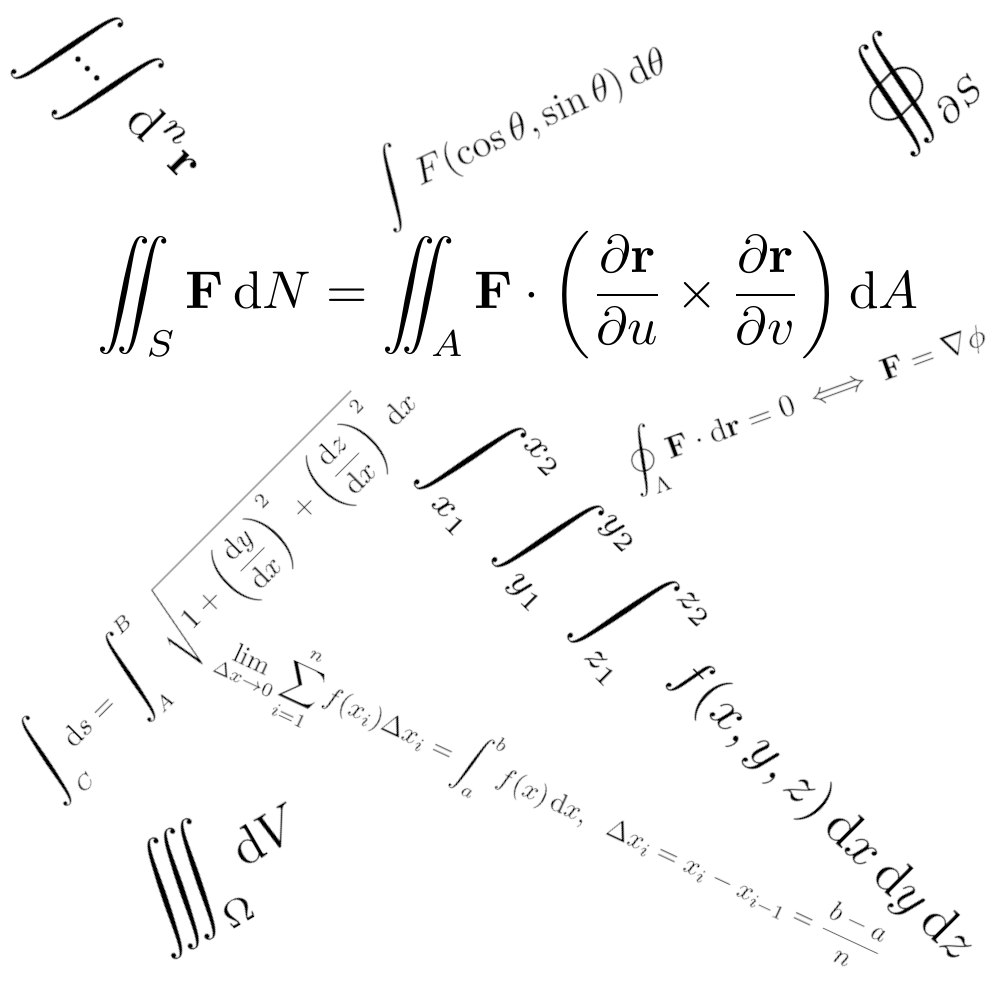
\includegraphics[width=0.9\linewidth]{TitlePhoto.png}
\end{figure*}

\pagebreak

\tableofcontents

\pagebreak

\section{Esipuhe}

\subfile{osiot/1_esipuhe}

\pagebreak

\section{Oppaassa käytetyt merkinnät}

\subfile{osiot/2_merkinnat}

\pagebreak

\section{Integraalien perusominaisuuksia}

\subfile{osiot/3_perusominaisuuksia}

\pagebreak

\section{Yhden muuttujan funktioiden integrointi}

\subfile{osiot/4_yhden_muuttujan_funktiot}

\pagebreak

\section{Kahden ja kolmen muuttujan funktioiden integrointi}

\subfile{osiot/5_monen_muuttujan_funktiot}

\pagebreak

\section{Numeerinen integrointi}

\subfile{osiot/6_numeerinen_integrointi}

\pagebreak

\section{Integraalien sovelluksia}

\subfile{osiot/7_sovelluksia}

\pagebreak











%
\end{document}
